\documentclass[a4paper, oneside, openany, dvipsnames, table]{article}
\usepackage[utf8]{inputenc}

%\usepackage{cm-super}

\usepackage{lmodern}
\usepackage[T1]{fontenc}
\usepackage[italian]{babel}
\usepackage{stile}


\begin{document}
\copertina
\tableofcontents
\newpage
\section{Introduzione}
	\input{sez/Introduzione.tex} %può anche rimanere vuoto
	\subsection{Abstract}
		Il progetto \emph{LumBooks}, svolto come finalità del corso di Tecnologie Web nell'anno accademico 2018-2019,
 si propone di implementare un sito Internet per la compravendita di materiale universitario tra studenti.\\
 Il nome "LumBooks", infatti, nasce dall'insieme delle parole Lum (che fa riferimento all'aula Lum250 del complesso Paolotti, dove si svolgono le lezioni del corso di studio di Informatca) e books.\\
Per conseguire lo scopo stabilito, la natura del sito è fortemente interattiva. Per i visitatori del sito è possibile infatti registrarsi e creare il proprio account personale, grazie al quale l'utente può cercare e vendere il materiale di studio che desidera, valutando offerte di altri utenti del sito.\\
Nonostante ciò la registrazione al sito non è obbligatoria, e nel caso un visitatore non volesse iscriversi il sito ha in qualsiasi caso funzionalità informative, in quanto permette comunque al visitatore esterno di cercare un determinato libro visualizzando le offerte che il sito propone.\\

Il sito è stato sviluppato con l’intenzione di essere poi pubblicato in internet, dunque si
è data molta importanza alla sua usabilità, rispettando gli standard W3C, la separazione tra struttura, presentazione, comportamento e le regole di accessibilità richieste.
	\subsection{About us}
		\input{sez/Introduzione/About_us.tex}
	
\newpage
\section{Analisi}
	\input{sez/Analisi.tex}
	\subsection{Studio dell'utenza finale}
		Il progetto LumBooks si propone come mezzo intermediario all'interno di in una compravendita di materiale universitario tra gli studenti; pertanto quest'ultimi saranno l'utenza finale primaria del sito, o comunque soggetti legati all'ambito accademico. \\ 
Nel particolare inizialmente la piattaforma viene pensata per essere destinata a studenti frequentanti il corso di studi di Informatica presso l'università di Padova (tant'è che il catalogo contiene prettamente libri appartenenti a questo corso), ma in futuro il sito potrebbe espandersi e rivolgersi a qualsivoglia studente frequentante una qualsiasi università.\\
In prospettiva di una futura crescita, quindi, l'utente finale potrebbe non essere specializzato o pratico di strumenti informatici, dal momento che potrebbe provenire da diverse facoltà. Per questo è necessario adottare un linguaggio informale, semplice e di facile intuizione, che possa essere compreso dalla maggior parte delle persone. Lo stesso discorso vale per il layout e la struttura del sito, che si prefiggono di essere intuitivi e veloci, rispettando le principali convenzioni del web.\\

	\subsection{Casi d'uso}
		\input{sez/Analisi/Casi_Uso.tex}
		\subsubsection{Utente generico}
			Definiamo \textit{generico} un utente che:
\begin{itemize}
	\item visita il sito senza possedere un account Lumbooks;
	\item visita il sito senza effettuare la login;
\end{itemize}

L'utente generico dispone dei seguenti casi d'uso:
\begin{itemize}
	\item \hyperref[par:VisHome]{Visualizzazione Homepage del sito (\ref{par:VisHome}});
	\item \hyperref[par:VisLibriVendita]{Visualizzazione dei libri correntemente in vendita nel sito (\ref{par:VisLibriVendita}});
	\item \hyperref[par:VisLibriCatalogo]{Visualizzazione dei libri appartenenti al catalogo del sito(\ref{par:VisLibriCatalogo}});
	\item \hyperref[par:RicercaLibro]{Ricerca di uno specifico libro tra quelli in vendita (\ref{par:RicercaLibro}});
	\item \hyperref[par:SpecLibro]{Visualizzazione di un particolare libro in vendita (\ref{par:SpecLibro}});
	\item \hyperref[par:VisAbout]{Visualizzazione pagina "Chi siamo" (\ref{par:VisAbout}});	
	\item \hyperref[par:Reg]{Registrazione (\ref{par:Reg}});
	\item \hyperref[par:Login]{Login (\ref{par:Login}}).
\end{itemize}

\paragraph{Visualizzazione Homepage del sito}\mbox{}\\
\label{par:VisHome}
L'utente generico può entrare nella Homepage in diversi modi:
\begin{itemize}
	\item Se è appena entrato nel sito è la prima pagina che viene visualizzata;
	\item Se si trova in un'altra pagina, può raggiungere la Homepage cliccando la sezione "Home" nella navbar;
	\item Se si trova in un'altra pagina, può raggiungere la Homepage cliccando sopra la scritta "Lumbooks" presente nell'header;
\end{itemize}
All'interno di questa pagina l'utente può apprendere le principali funzionalità del sito e visionare le ultime offerte inserite inserite (nell'apposita sezione in basso "Le nostre ultime offerte!")



\paragraph{Visualizzazione dei libri correntemente in vendita}\mbox{}\\
\label{par:VisLibriVendita}
L'utente generico entra nella pagina di visualizzazione dei libri in vendita cliccando la sezione "in vendita" presente nella navbar".\\
I libri visualizzati in questa sezione possono essere appartenenti al catalogo Lumbooks o esterni a esso. A seconda della tipologia di libro vi sono delle caratteristiche obbligatorie e altre opzionali. Ogni libro quindi è visualizzato all'interno di una scheda, che ne contiene le seguenti caratteristiche (a prescindere che si tratti di un libro appartenete al catalogo o meno):
\begin{itemize}
	\item Titolo (obbligatorio, sempre presente);
	\item Autore (obbligatorio, sempre presente);
	\item Prezzo (obbligatorio, sempre presente);
	\item ISBN (presente opzionalmente);
	\item Foto del libro (presente opzionalmente);
\end{itemize}

\paragraph{Visualizzazione di un particolare libro in vendita}\mbox{}\\
\label{par:SpecLibro}
Nel caso l'utente volesse ulteriori informazioni su un determinato libro, il titolo del libro presente nella scheda è un link che indirizza a un'altra pagina, dove sono visualizzati in maniera più specifica le caratteristiche del libro. Tra le caratteristiche aggiuntive in questa pagina possiamo trovare:
\begin{itemize}
	\item Editore;
	\item Che tipo di materiale di studio è (libro, dispense..);
	\item Anno di pubblicazione;
	\item Edizione;
	\item Casa editrice;
	\item Una breve descrizione del libro;
	\item Recapiti del venditore.
\end{itemize}

\paragraph{Visualizzazione dei libri del catalogo}\mbox{}\\
\label{par:VisLibriCatalogo}
L'utente generico entra nella pagina di visualizzazione dei libri appartenenti al catalogo LumBooks cliccando la sezione "catalogo" presente nella navbar".\\
All'interno della pagina sono visualizzati i libri del catalogo, all'interno di schede analoghe a quelle riportate nella pagina "In vendita".\\
Le caratteristiche qui riportate per ogni libro sono:
\begin{itemize}
	\item Titolo;
	\item Autore;
	\item Casa editrice;
	\item Corso a cui fanno riferimento;
\end{itemize}
Anche in questa pagina il titolo del libro presente in ogni scheda è un link: cliccandolo si viene reindirizzati alla pagina "risultati della ricerca", che visualizza tutti i libri in vendita corrispondenti al libro di catalogo di cui si è selezionato il titolo. Per esempio se clicco il titolo del libro "Programmazione: semplice è bello" vengo reindirizzato alla pagina di risultati che visualizza tutte le offerte di questo libro presenti nel sito.

\paragraph{Ricerca di un libro tra quelli in vendita}\mbox{}\\
\label{par:RicercaLibro}
L'utente generico entra nella pagina di ricerca dei libri in vendita cliccando la sezione "Cerca un libro" presente nella navbar".\\
La pagina offre all'utente un motore di ricerca statico che permette di ricercare determinati materiali all'interno del sito.\\
I parametri per la ricerca sono:
\begin{itemize}
	\item Titolo;
	\item Autore;
	\item Corso;
	\item Editore;
	\item ISBN;
	\item Parola chiave;
\end{itemize}
L'utente può decidere quali campi compilare a seconda del grado di precisione della ricerca che vuole effettuare: nessun campo è a compilazione obbligatoria. Inoltre la compilazione dei campi non è case sensitive.\\
Una volta compilati i campi l'utente preme il tasto "Cerca" ed effettua la ricerca. Gli esiti possibili sono due:
\begin{itemize}
	\item La ricerca è andata a buon fine, quindi viene visualizzata una pagina contenente tutti i risultati corrispondenti a tale ricerca. La modalità di visualizzazione dei risultati è analoga a quella presente nella sezione "in vendita": ogni libro è contenuto in una scheda che ne descrive le caratteristiche.;
	\item La ricerca non sortisce risulati: non esistono corrispondenze per la ricerca effettuata: viene visualizzato un seganle di errore che invita a eseguire un'altra ricerca;
	
\end{itemize}

\paragraph{Visualizzazione pagina "Chi siamo"}\mbox{}\\
\label{par:VisAbout}
L'utente generico entra nella pagina di visualizzazione dei libri in vendita cliccando la sezione "chi siamo" presente nella navbar".\\
All'interno di questa pagina statica sono contenute le informazioni riguardanti i componenti del gruppo e la nascita del progetto Lumbboks.

\paragraph{Registrazione}\mbox{}\\
\label{par:Reg}
L'utente generico entra nella pagina di registrazione cliccando la sezione "Registrati" presente nell'header".\\
La pagina offre all'utente generico la possibilità di creare il proprio account personale LumBooks. Un utente può possedere più account LumBooks, a patto che vengano registrati con email diverse.\\
Per effettuare la registrazione l'utente deve inserire una serie di dati, alcuni obbligatori (quelli contrassegnati con *) e altri opzionali. al termine dell'inserimento l'utente preme il tasto registrati, e gli esiti possibili sono due:
\begin{itemize}
	\item La registrazione è andata a buon fine, l'inserimento dei dati è avvenuto in maniera corretta. Viene visualizzato un messaggio che indica che l'operazione si è conclusa correttamente e si viene reindirizzati alla homepage ;
	\item La registrazione non è andata a buon fine, e questo può essere dovuto a diverse motivazioni. Se i dati inseriti non sono corretti (per esempio email nel formato sbagliato, ripetizione della password non coincide) vengono visualizzati dei messaggi di errore che indicano il/i problemi e in seguito si invita a reinserire i dati sbagliati (i dati inseriti correttamente rimangono nei campi di compilazione);
\end{itemize}

\paragraph{Login}\mbox{}\\
\label{par:Login}
L'utente generico entra nella pagina di login cliccando la sezione "Accedi" presente nell'header".\\
La pagina offre all'utente già in possesso di un account Lumbooks la possibilità di accedervi, inserendo le proprie credenziali (email e password). Gli esiti dell'inserimento possono essere due:
\begin{itemize}
	\item L'inserimento dei dati è corretto; l'utente accede correttamente al suo account Lumbooks. Al termine dell'inserimento viene reindirizzato alla Homepage;
	\item L'inserimento dei dati non è corretto; l'utente non accede al suo account Lumbooks. Possono essere diverse le casistiche che portano a tale risultato: password e/o email non corretta. In ogni caso viene indicato all'utente qual'è il problema, attraverso appositi messaggi di errore. 
\end{itemize}
L'inserimento inoltre contiene un controllo per quanto riguarda l'inserimento dell'email: viene controllato che il formato sia effetivamente quello di un email, e in caso contrario viene segnalato all'utente.




		\subsubsection{Utente loggato}
			Definiamo \textit{loggato} un utente che:
\begin{itemize}
	\item Ha eseguito con successo il login;
	\item Si è registrato con successo, ed è quindi stato rimandato alla home. In questo caso, il login è avvvenuto automaticamente.
\end{itemize}

L'utente loggato eredita tutti i casi d'uso dell'utente generico, eccetto:
\begin{itemize}
	\item Registrazione;
	\item Login;
\end{itemize}

L'utente loggato dispone, inoltre, dei seguenti casi d'uso:
\begin{itemize}
	\item \hyperref[par:Inserimento]{Inserimento di un nuovo libro (\ref{par:Inserimento}});
	\item \hyperref[par:VisLibriUt]{Visualizzazione dei propri libri in vendita e venduti (\ref{par:VisLibriUt}});
	\item \hyperref[par:ModLibro]{Modifica di un proprio libro in vendita (\ref{par:ModLibro}});
	\item \hyperref[par:VendLibro]{Marcatura di un proprio libro in vendita come venduto (\ref{par:VendLibro}});
	\item \hyperref[par:RimuoLibro]{Rimozione di un proprio libro dal sito (\ref{par:RimuoLibro}});
	\item \hyperref[par:VisDati]{Visualizzazione dei propri dati di iscrizione al sito (\ref{par:VisDati}}).
\end{itemize}

\paragraph{Inserimento di un nuovo libro}\mbox{}\\
\label{par:Inserimento}
L'utente loggato entra nella pagina di inserimento libri clickando su \textit{Inserisci} nella navbar. Nella pagina di inserimento l'utente può scegliere se scegliere di inserire:
\begin{itemize}
	\item Una propria istanza di un libro già in catalogo: in questo modo, molto dei campi saranno già precompilati. Clicando sul menù a tendina, l'utente avrà a dispozione i titoli dei volumi selezionabili.
	\item Un libro non presente in catalogo: l'utente dovrà inseirire più campi rispetto alla prima opzione, ma potrà insiere un libro a libera scelta.
\end{itemize}
In caso l'utente inserisca un campo dati non conforme al formato atteso (ex. ISBN con lunghezza diversa da 13, prezzo con tre cifre decimali), sarà di ciò dal sito, e verrà invitato a insere i dati nel modo corretto.
Se, invece, l'inserimento è avvenuto con successo, il sito infomerà l'utente e lo reindirizzerà alla home.

\paragraph{Visualizzazione dei propri libri in vendita e venduti}\mbox{}\\
\label{par:VisLibriUt}
L'utente loggato entra nella pagina di visualizzazione libri clickando su \textit{I miei Libri} nella navbar. Da qui, l'utente può visualizzare i proprio libri divisi fra \textit{In vendita} e \textit{Venduti}, e rappresentati tramite delle card simili a quelle presenti nelle schermate di ricerca libro £££££££££££££AGGIUNGERE LINK££££££££££, ma presentanti tre bottoni:
\begin{itemize}
	\item \hyperref[par:ModLibro]{Modifica (\ref{par:ModLibro})};
	\item \hyperref[par:VendLibro]{Venduto (\ref{par:VendLibro})};
	\item \hyperref[par:RimuoLibro]{Rimuovi (\ref{par:RimuoLibro})}.
\end{itemize}
L'utente inoltre, oltre alle informazioni che vedrebbe nella pagina di ricerca del libro, ha a dispozione la data di aggiunta del libro stesso.

\paragraph{Modifica di un proprio libro in vendita}\mbox{}\\
\label{par:ModLibro}
Nella schermata di visualizzazione dei propri libri, l'utente preme il tasto \textit{Modifica} sulla card di un libro in vendita. Viene quindi caricata la pagina di modifica del libro, molto simile a quella di inserimento. L'utente, quindi, modifica i campi a sua scelta, e poi conferma i cambiamenti apportarti. Se tutto è andato bene, il sito reindirizza l'utente ai propri libri; in caso contrario, l'utente viene informato dell'errore e invitato a riprovare.

\paragraph{Marcatura di un proprio libro in vendita come venduto}\mbox{}\\
\label{par:VendLibro}
Nella schermata di visualizzazione dei propri libri, l'utente preme il tasto \textit{Venduto} sulla card di un libro in vendita. Ciò comporta lo spostamento del libro nella sezione \textit{Libri Venduti} tramite un refresh della pagina. Un libro che viene segnato come venduto non può essere rimesso in vendita, e rimangono disponibili solo le seguenti operazioni:
\begin{itemize}
	\item Visualizzazione del libro £££££££INSERIRE LINK£££££££££££;
	\item \hyperref[par:RimuoLibro]{Rimozione del libro (\ref{par:RimuoLibro})}.
\end{itemize}

\paragraph{Rimozione di un proprio libro dal sito}\mbox{}\\
\label{par:RimuoLibro}
Nella schermata di visualizzazione dei propri libri, l'utente preme il tasto \textit{Rimuovi} sulla card di un libro. Il libro viene rimosso dal sito tramite un refresh della pagina, e non è più possibile reperirlo nella piattaforma.

\paragraph{Visualizzazione dei propri dati di iscrizione al sito}\mbox{}\\
\label{par:VisDati}
L'utente, una volta loggato, visuallizza la propria immagine profilo nella navabar. Se invece, al momemento dell'iscrizione, l'utente avesse scelto di non caricarne una, visualizzerà un'immagine generica.
Per visualizzare il resto dei suo dati, l'utente clicca il link \textit{I miei dati} sulla navbar, e viene portato a una pagina riassuntiva con le sue informazioni.








		\subsubsection{Amministratore}
			L'amministratore è l'utente caratterizzato dall'indirizzo email fittizio \texttt{admin@admin.com}. Eredita tutti gli use case di \textit{utente loggato}, e dispone di alcune funzionalità extra:
\begin{itemize}
	\item \hyperref[par:PanAm]{Accesso al pannello amministratore (\ref{par:PanAm})};
	\item \hyperref[par:InsCat]{Inserimento libri in catalogo (\ref{par:InsCat})};
	\item \hyperref[par:RimCat]{Rimozione libri da catalogo (\ref{par:RimCat})};
\end{itemize}

\paragraph{Accesso al pannello amministratore}\mbox{}\\
\label{par:PanAm}
L'amministratore può accedere al pannello amministratore cliccando il link \textit{Pannello Amministratore} sulla navbar. Mentre l'utente normale viene bloccato da un messaggio di errore, l'amministratore visualizza il pannello che consiste in:
\begin{itemize}
	\item Un form per l'inserimento nei libri in catalogo;
	\item La lista dei libri in catalogo, con annessi id interno del database e bottone \textit{Elimina}.
\end{itemize}

\paragraph{Inserimento libri in catalogo}\mbox{}\\
\label{par:InsCat}
Una volta nel pannello, l'amministratore può usare il form presente per inserire libri nel catalogo. Se inserisce dati validi, la pagina verrà aggiornata, e sarà possibile visualizzare a schermo la nuova entry; altrimenti verrà mostrato un messaggio d'errore.

\paragraph{Rimozione libri da catalogo}\mbox{}\\
\label{par:RimCat}
Una volta nel pannello, l'amministratore può decidere di rimuovere uno qualsiasi dei libri dal catalogo premendo il tasto \textit{Elimina}. Dopo un aggiornamento automatico della pagina, tale libro non sarà più visibile. Da notare che tale operazione non elimina le istanze dei libri presenti nel database, che verranno invece dissociate dal libro in catalogo durante la procedura di eliminazione di quest'ultimo.


\newpage
\section{Progettazione}
	\input{sez/Progettazione.tex}
	\subsection{Obiettivi}
		Nello sviluppo del sito sono stati perseguiti alcuni obiettivi, elencati in seguito.

\begin{itemize}
	\item \textbf{Separazione struttura-presentazione:} Questo obiettivo è senza ombra di dubbio da considerasi il più importante, in quanto il suo raggiungimento comporta una maggior facilità nel soddisfare anche gli altri obiettivi. I contenuti del sito e la loro struttura devono essere separati dalla parte di presentazione grafica: si sono quindi definite le componenti di stile nei fogli CSS, mentre il contenuto è perlopiù gestito da PHP e HTML.
	
	\item \textbf{Accessibilità: } Il sito deve poter essere fruibile agevolmente dal maggior numero utenti possibile, compresi quelli con gravi disabilità visive e/o motorie. Per raggiungere tali obiettivi, sono state adottate varie misure, fra i quali citiamo le più significative:
	\begin{itemize}
		\item TabIndex sui form;
		\item Testo alternativo per le immagini;
		\item Testi e link con buoni livelli di contrasto;
	\end{itemize}
	
	\item \textbf{Flessibilità:} Il sito deve essere consultabile da varie tipologie di dispositivi, smartphone compresi. Deve, inoltre, essere adattabile a differenti dimensioni di schermo con il minor sforzo possibile.
	
	\item \textbf{Facilità d'uso:} Per rendere il sito maggiormente intuitivo per l'utente finale si è scelto di rispettare le convenzioni del web, anteponendo, quando possibile, queste ultime all'estetica del sito. Un esempio di tale scelta si può notare nei link: essi sono di colore blu sottolineato come l'utente è solito aspettarsi, e diventato viola se già visitati. Alcuni link, posti su sfondo azzurro, sono invece bianchi per avere un livello di contrasto sufficiente.
\end{itemize}
	%parlo di separazione struttura contenuto ecc, accessibilita.....
	\subsection{Layout}
		\begin{figure}
	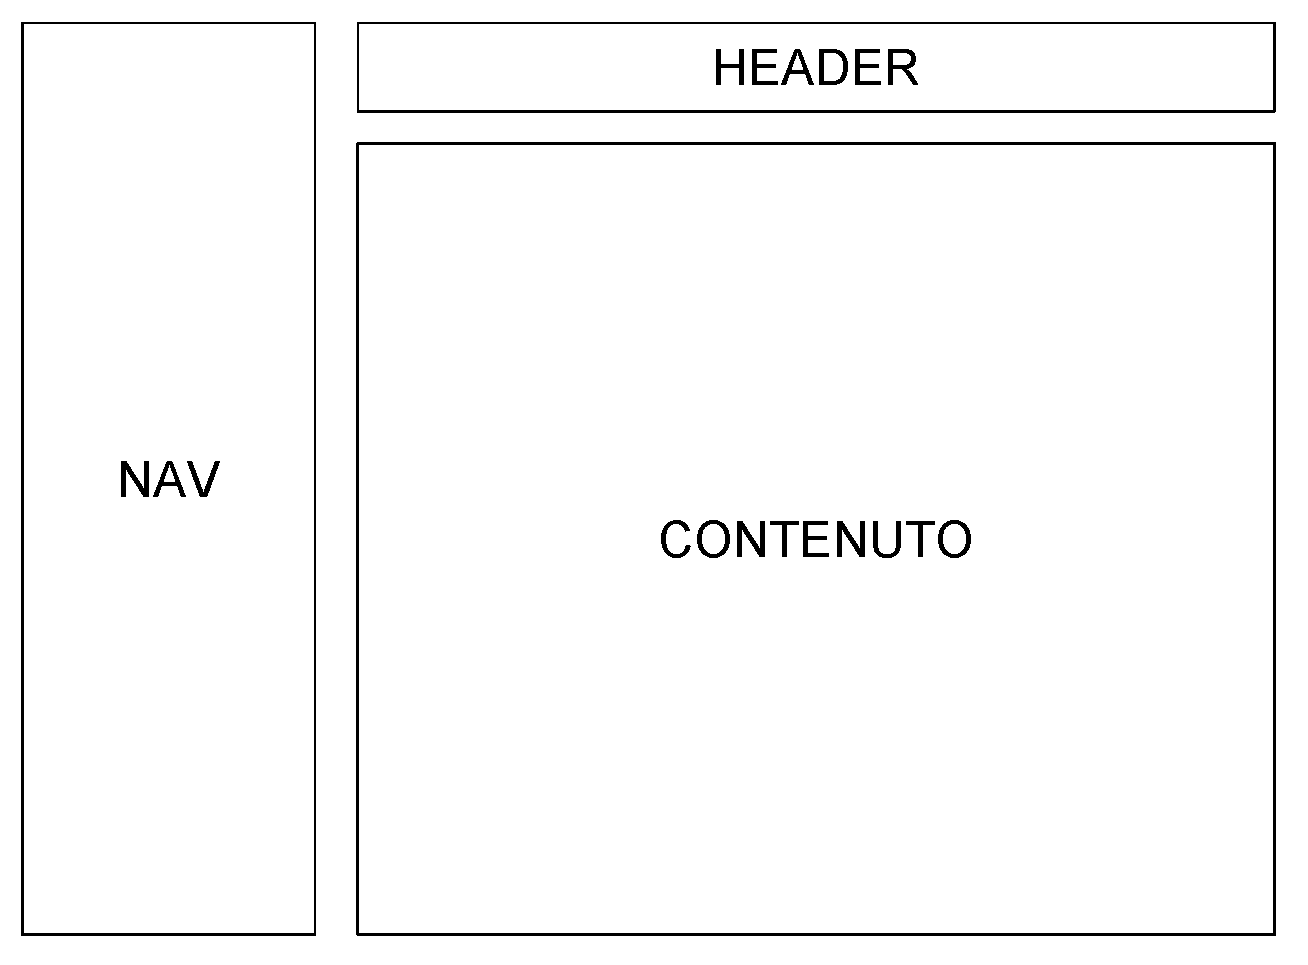
\includegraphics[width=1\linewidth]{sez/Progettazione/layout-base.pdf}
	\caption{Layout di una generica pagina del sito}
	\label{Fig:layoutBase}
\end{figure}

Per il sito è stato scelto un \textit{layout a tre pannelli}, come illustrato in \autoref{Fig:layoutBase}. Tale modello garantisce una superiore flessibilità e facilità di modifica in caso di aggiunta o rimozione di contenuti, e una maggiore adattabilità a taglie di schermo differenti. Ogni pagina del sito segue questo schema.
		\subsubsection{Resize e Mobile}
			Essendo tutte le unità di misura del sito definite in \textit{em}, è possibile cambiare la dimensione del font alla base del sito per far scalare di conseguenza l'interfaccia, con buoni risultati.\\
Tuttavia, sono stati necessari alcuni accorgimenti per avere un'interfaccia mobile utilizzabile, il più radicale dei quali è stato inserire una navbar a scomparsa. Il risultato è visibile in \autoref{Fig:layoutMobile}. Ciò è stato ottenuto mediante l'inserimento di una burger icon nell'header: un tap su tale icona apre la navbar, che si sovrappone al resto della pagina. Il menù si può quindi chiudere attraverso la x posta in alto a destra.\\

\begin{figure}
	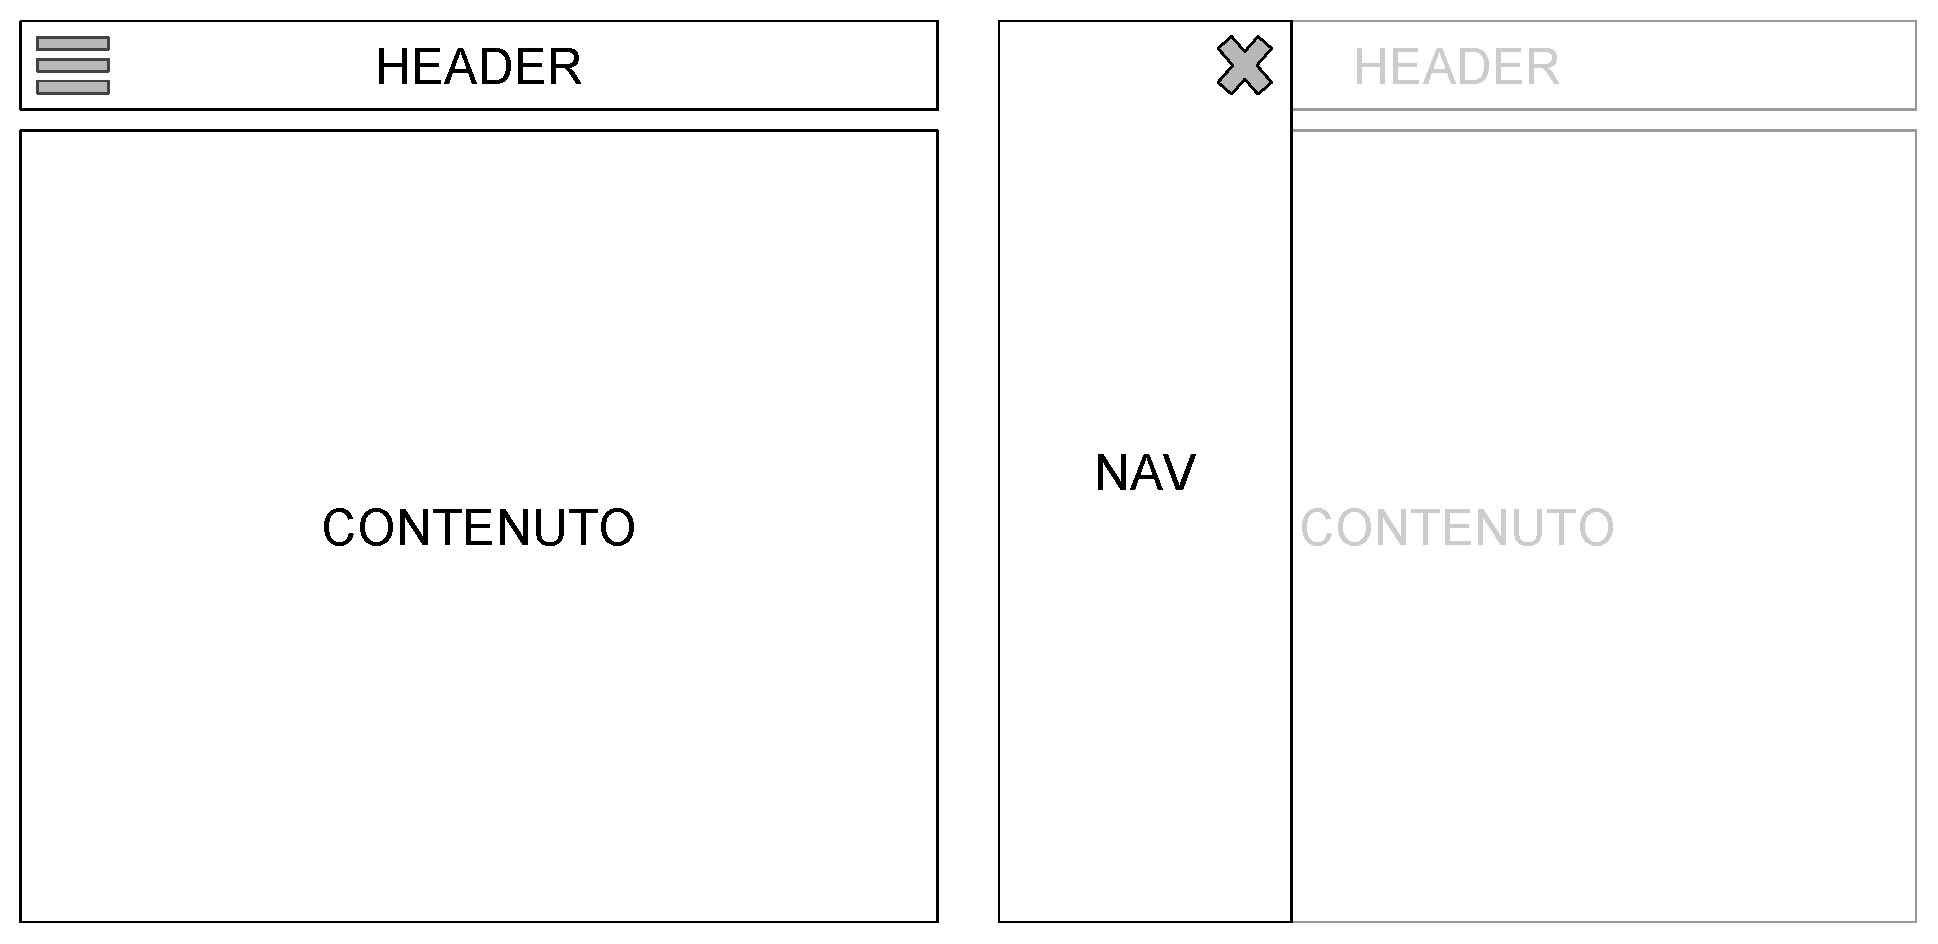
\includegraphics[width=1\linewidth]{sez/Progettazione/Layout/layout-mobile.pdf}
	\caption{Layout di una generica pagina del sito in versione mobile, a sinistra con navbar nascosta, a destra con navbar aperta}
	\label{Fig:layoutMobile}
\end{figure}

Altro dettaglio che cambia a seconda della dimensione della finestra è la visualizzazione dei risultati di ricerca di un libro, come rappresentato in \autoref{Fig:searchItems}. I risultati della ricerca vengono mostrati cercando di avere un buon compresso fra leggibilità e necessità di scrolling.

\begin{figure}
	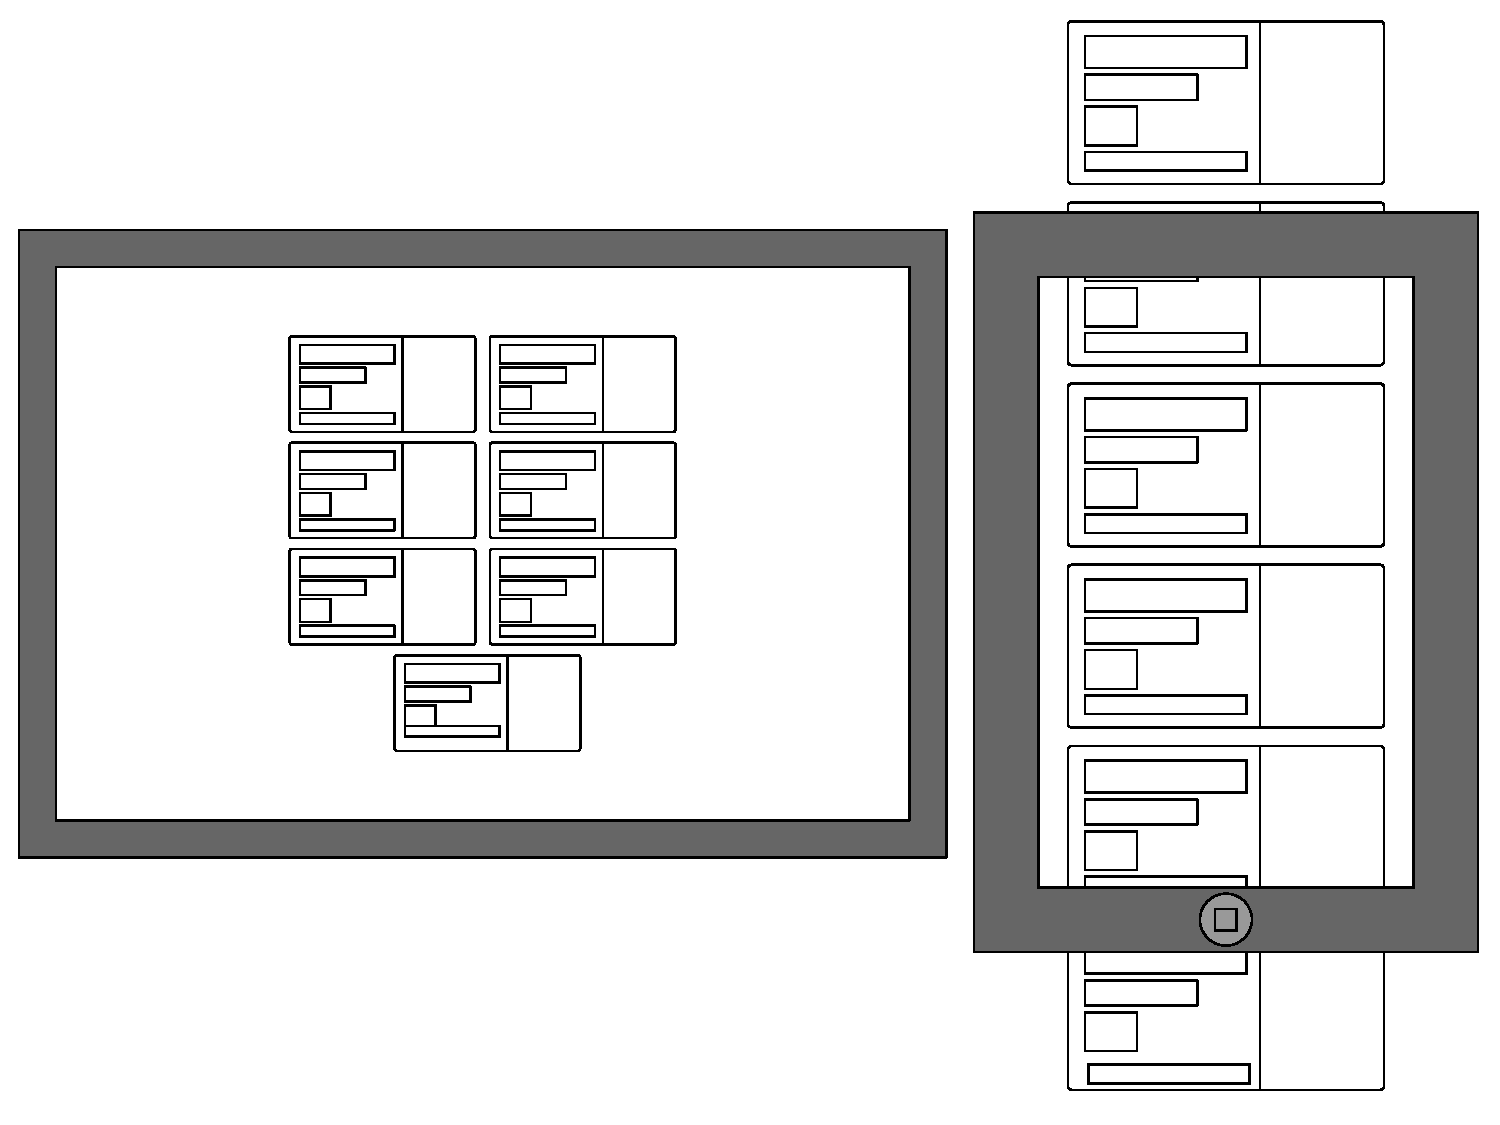
\includegraphics[width=1\linewidth]{sez/Progettazione/Layout/Search-items.pdf}
	\caption{Layout dei risultati di ricerca desktop (sinistra) e mobile (destra)}
	\label{Fig:searchItems}
\end{figure}
	\subsection{Accessibilità}
		\input{sez/Progettazione/Accessibilita.tex}
		\subsubsection{Trasformazione elegante}
			Il primo punto per progettare un sito web accessibile è garantire una trasformazione elegante delle pagine web. Per assicurarsi ciò si è innanzitutto separato la gli aspetti riguardanti contenuto, presentazione e struttura, come si è già discusso precedentemente. Successivamente sono state fornite equivalenti testuali per ogni media, permettendo anche agli utenti non vedenti di accedere alle informazioni attraverso l'udito. Inoltre le pagine sono responsive, poiché si adattano a seconda delle dimensioni dello schermo dell'utilizzatore, grazie al vasto utilizzo di dimensioni relative nei fogli di stile e grazie all'utilizzo di punti di rottura che ne facilitano la progettazione multi-piattaforma.
		\subsubsection{Tastiera e scorciatoie}
			Per permettere agli utenti che utilizzano dispositivi differenti dal mouse e per garantire scorciatoie, in particolare modo alle categorie di utenti svantaggiate, sono stati utilizzati diversi strumenti:
\begin{itemize}
	\item \textbf{Fieldset:}tutti gli input in un form sono stati raggruppati in fieldset, ovviamente corredato corredato da una leggenda opportuna;
	\item \textbf{Tabindex:}per ogni form sono stati ridefiniti i tabindex, permettendo all'utente di spostarsi da un input al successivo, e stabilendo un opportuno ordine di tabulazione;
	\item \textbf{Accesskey: }vi è una scorciatoia da tastiera che consente di accedere alla pagina "Chi siamo"; poiché non è possibile far conoscere le scorciatoie in anticipo, è stato inserito un indizio nella barra di navigazione.
\end{itemize}
		\subsubsection{Schema colori}
			La scelta dei colori ha un impatto fondamentale per quanto riguarda l'accessibilità del sito. Innanzitutto è stato garantito un contrasto elevato per facilitare la lettura del contenuto e differenziare i diversi elementi strutturali, mantenendo sempre una coerenza nelle scelte che crediamo possa facilitare la formazione di una mappa mentale. In particolare, i link sono facilmente riconoscibili, in quanto ci siamo attenuti alle convenzioni ben consolidate e abbiamo garantito una loro rappresentazione uniforme nel sito. Sono quindi facilmente distinguibili i link già visitati.
L'unica eccezione è data dagli elementi della barra di navigazione: in questo caso i bottoni vengono evidenziati al passaggio del puntatore attraverso il selettore :hover presente in CSS3. Naturalmente, da una determinata sezione del menu non sarà possibile cliccare nuovamente sulla stessa sezione, e ciò è facilmente riconoscibile in quanto tale link diventa un semplice contenuto testuale.
	\subsection{Schema organizzativo}
		Il contenuto del sito è relativamente omogeneo e risulta organizzato come una collezione di processi differenti. Per questi motivi è stato scelto uno schema organizzativo ambiguo orientato al \textit{task}. Crediamo che questa scelta sia la più appropriata in quanto vi è un numero limitato di compiti ad alta priorità, come per esempio la ricerca o l'inserimento di libri.\\
L'utente, dopo aver selezionato il \textit{task} iniziale, sarà guidato fino al raggiungimento del proprio obiettivo attraverso il riempimento di informazioni negli input opportuni e secondo una struttura sequenziale, sempre all'interno del sito. Ciò permette anche di rendere l'accesso ai contenuti il più semplice possibile, evitando possibili sovraccarichi cognitivi.
	%principi_web_design slide numero 16

\newpage
\section{Implementazione}
	\input{sez/Implementazione.tex}
	\subsection{Linguaggi e strumenti}
		\input{sez/Implementazione/LinguaggiEStrumenti.tex}
		\subsubsection{HTML 5}
			Il gruppo ha utilizzato il linguaggio HTML5\footnote{https://www.w3.org/TR/2017/REC-html52-20171214/} per la struttura del sito, mantenendo comunque la compatibilità con XHTML\footnote{https://www.w3.org/TR/2015/REC-xhtml-rdfa-20150317/}. Questo permette al sito di funzionare sui browser più obsoleti e migliora la comprensibilità del codice.\\
Per assicurare un codice corretto, sono state seguite le linee guida del corso di TecWeb e W3C\footnote{https://www.w3.org/standards/webdesign/htmlcss}. Il codice è stato validato utilizzando il tool di validazione W3C\footnote{https://validator.w3.org/\#validate\_by\_uri}.\\
Le regole più importanti sono:
\begin{itemize}
    \item \textbf{Chiusura tag:} ogni tag deve essere chiuso(<tag></tag oppure <tag/>);
    \item \textbf{Tag intestazione:} per ogni sezione (body, div, section) ogni tag di intestazione (h1,h2,...) deve partire sempre da h1;
    \item \textbf{Metatag:} nella sezione header, devono essere inseriti i metatag necessari per migliorare l'accessibilità verso i motori di ricerca. Questo permette al sito di avere una migliore visibilità in internet; 
    \item \textbf{Separazione struttura presentazione comportamento:} il codice HTML non deve contenere CSS o script. Questi devono essere scritti in file separati e importati nell'header;
    \item \textbf{Struttura:} il codice HTML non deve sostituire il CSS, quindi non può contenere elementi per la presentazione;
    \item \textbf{Tabelle:} Le tabelle devono essere evitate quando possibile.
\end{itemize} 
		\subsubsection{PHP}
			Il linguaggio di programmazione PHP è stato usato per il backend e per la composizione di codice HTML.\\
I file coinvolti nella parte di struttura sono:
\begin{itemize}
    \item \textbf{htmlMaker.php:} contiene una serie di funzioni utili alla costruzione del sito:\label{htmlmaker}
        \begin{itemize}
            \item \textbf{generateBookCollection} costruisce una collezione di libri. Prende come parametri \textit{listaLibri} (array contenente una lista di libri) e \textit{lista\_bottoni} (opzionale. Rappresenta una lista di bottoni da aggiungere al libro). Questa funzione utilizza singleItem e singleItemWithButtons che generano un singolo libro;
            \item \textbf{navbar} costruisce la navbar; questo è l'elemento più mutabile del sito, quindi viene costruito interamente attraverso del codice php;
            \item \textbf{pagina\_messaggio} costruisce una pagina molto semplice, usato principalmente per pagine di errore. Prende come parametri titolo, sottotitolo ed extra (opzionale).
        \end{itemize}
    \item \textbf{"nomepagina".php:} (esempio: home.php, login.php) sono i file che costruiscono le pagine del sito. Utilizzano le funzioni di htmlMaker e il rispettivo file html (es: home.php usa home.html) che contiene l'effettivo html; 
\end{itemize}
Il gruppo ha deciso di utilizzare codice PHP rivolto alla struttura del sito, perché alcuni contenuti strutturali del sito sito cambiano se l'utente è sconosciuto oppure ha effettuato l'accesso. Le differenze sono:
\begin{itemize}
    \item I bottoni per effetturare il login vengono sostituiti dal bottone di logout;
    \item Alla navbar laterale vengono aggiunti l'immagine di profilo dell'utente e i link per accedere alla configurazione del suo account;
    \item Alla narbar laterale viene aggiunto il pulsante (inserisci) per la vendita di un libro;
\end{itemize}
L'utilizzo del PHP per la struttura ha permesso anche le seguenti caratteristiche:
\begin{itemize}
    \item \textbf{Unico header, navbar e footer}: L'header, la navbar e il footer sono gli stessi per ogni pagina. Questo permette una maggiore manuntenibilità del sito, in quanto una modifica a un file si riflette su tutte le pagine del sito web;
    \item \textbf{Link circolari:} Un solo codice per tutti i file genera dei link circolari, che vengono rimossi tramite codice PHP (esempio: per rimuovere i link circolari dalla home si utilizza questa funzione: str\_replace('<a href="home.php">','<a>',"\- link alla pagina home \-");
    \item \textbf{Riempire i campi in caso di errore:} se prova a inserire un libro ma ci sono degli errori (che passano i controlli JavaScript), tramite PHP vengono riempiti i campi corretti, permettendo all'utente di non doverli inserire nuovamente;
    \item \textbf{Costruzione card dei libri:} le pagine che contenegono dei libri cambiano a seconda dei libri presenti nel database. Per questo motivo, il file \textit{htmlMaker.php} contiene le funzioni \textit{singleItem} e \textit{singleItemWithButtons} per costruire le card dei libri, a partire da un risultato SQL.
\end{itemize}
La parte di backend gestisce principalmente le richieste di modifica al database da parte degli utenti del sito:
\begin{itemize}
    \item \textbf{sql\_wrapper:} il file \textit{sql\_wrapper} contiene delle funzioni per accedere al database; lo scopo di questo file è semplificare l'accesso al database per gli altri;  
    \item \textbf{Login:} l'accesso avviene attrraverso il file \textit{check\_login.php}, che, tramite l'sql\_wrapper, controlla se l'email e la password esistono. In caso positivo viene aperta la sessione;
    \item \textbf{Registrazione:} la registrazione avviene attrraverso il file \textit{new\_user.php}. Se la registrazione ha successo, viene fatto il login automatico;
    \item \textbf{Validazione campi:} il file \textit{validator.php} contiene delle funzioni utili alla validazione dei campi in registrazione, login, inserimento libri;
    \item \textbf{Sessione:} il file \textit{back\_end.php} contiene funzioni per capire se la sessione è aperta (quindi se il login è stato effettuato).
\end{itemize}
		\subsubsection{SQL}
			Sql è stato utilizzato per la codifica del database.
Il database è composto dalle seguenti tabelle:
\begin{itemize}
    \item \textbf{Utente:} contiene le credenziali appartenenti a un utente registrato al sito. Per proteggere la password, viene codificata in \textit{Pw\_Hash} tramite la funzione \textit{password\_hash} di php. Il \textit{codice\_identificativo} del libro è un numero che incrementa ad ogni libro inserito;
    \item \textbf{Libri\_Listati:} contiene i libri listati (catalogo);
    \item \textbf{Libri\_In\_Vendita:} contiene i libri che gli utenti mettono in vendita. Viene controllato che il \textit{prezzo} sia positivo, che lo \textit{stato} sia "Venduto","In Vendita" o "Prenotato" e che il \textit{tipo} sia "Libro","Slide","Appunti","Altro" o "Dispense";
\end{itemize}
		\subsubsection{JavaScript}
			Il linguaggio di programmazione Javascript è stato utilizzato per la parte di front end del sito.\\
Per ridurre il traffico di file, tutte le funzioni sono inserite in \textit{action.js}.
JS è stato utilizzato per:
\begin{itemize}
    \item convalidare i dati nella registrazione, durante l'inserimento di libri in vendita e mentre l'utente effettua il login;
    \item configurare bottone per chiudere e aprire la navbar laterale, assieme al CSS. 
\end{itemize}
	\subsection{Funzionamento generale}
		Ogni pagina è formata da tre elementi principali:
\begin{itemize}
    \item \textbf{header:} contiene il logo, il titolo e i bottoni \textit{accedi} e \textit{registrati} per un utente non autenticato, \textit{Logout} per un utente autenticato;
    \item \textbf{nav:} contiene i link per la navigazione. L'utente autenticato ha anche l'immagine di profilo e i link per il pannello del controllo. Viene generata da htmlMaker (vedere \ref{htmlmaker});
    \item \textbf{section:} contiene il contenuto principale del sito. Cambia per ogni pagina. Per la maggior parte dei casi, il contenuto di section corrisponde al contenuto della corrispondente pagina ".html" (es. section della Home è il contenuto di home.html). Il contenuto può essere diverso, se dipende dai dati inseriti nel database (card dei libri o i dati dell'utente nel pannello utente).
\end{itemize}
Il catalogo e i libri in vendita sono una unordered list (<ul class='books\_collection'>), creata da generateBookCollection come definito in \ref{htmlmaker}. Ogni libro è un elemento (<li class="search\_item">) con l' id uguale all'id del libro nel database (md5\_Hash). Gli altri elementi del libro sono un div contenete le informazioni dello stesso e l'immagine (se presente).\\
L'inserimento di un libro in vendita è permesso solamente a un utente registrato. L'utente può scegliere se il libro è nel catalogo (quindi i campi Titolo, Autore, Casa editrice, Corso non sono richiesti) oppure se non è presente. L'immagine del libro non è obbligatoria, se non presente viene mostrato un placeholder.
	\subsection{Separazione struttura-contenuto}
		Il gruppo ha considerato come fondamentale la separazione tra la struttura e il contenuto. Per questo fine, si è posto le seguenti regole:
\begin{itemize}
    \item \textbf{JavaScript non intrusivo:} tutto il codice JS è stato inserito in un file separato dai file Html e Php (\textit{action.js}), evitando quindi l'utilizzo di elementi come <div "onClick="funzione()"/>;
    \item \textbf{PHP non intrusivo:} anche se una parte del codice PHP genera codice HTML, la pagina finale non contiene elementi PHP. Inoltre, tutto il codice HTML che non proviene da un file viene scritto attraverso il comando "echo";
    \item \textbf{CSS non intrusivo:} come per JavaScript, anche tutto il codice CSS è stato inserito in un file dedicato (\textit{style.css}).
    \item \textbf{HTML solo per la struttura:} come accennato in \ref{struttura}, l'HTML non può contenere elementi di stile. L'HTML, quindi, \textbf{non} deve essere utilizzato in questi casi:
        \begin{itemize}
            \item usare una tabella per il layout (usare invece un layout responsive attraverso CSS);
            \item definire la dimensione, colore e stile generale del testo (usare invece classi e tagname corretti, per poi essere modificati con il CSS);
            \item usare le intestazioni (h1,h2,h3...) solo per definire la dimensione del testo;
            \item usare il <br/> per andare a capo;
        \end{itemize} 
\end{itemize} 
\textit{style.css} e \textit{action.js} sono state importate nell'\textit{head}.
	
\newpage
\section{Validazione}
	La validazione delle pagine è fondamentale per garantire un sito web accessibile e aderente agli standard. In particolare, sono stati utilizzati diversi strumenti per la validazione automatica del sito. Si noti che, poiché le pagine sono in php, abbiamo validato sia ogni singolo file del sito, sia il codice sorgente effettivo che produceva il php. Naturalmente le pagine in HTML5 sono state validate in XHTML,
	\subsection{Strumenti usati (da espandere)}
		Per la validazione dei file HTML sono stati utilizzati due servizi: TotalValidator\footnote{https://www.totalvalidator.com} e il validatore di W3C\footnote{https://validator.w3.org} . Per il CSS del sito è stato sfruttato un altro validatore sempre offerto dal W3C\footnote{http://www.css-validator.org}. Infine, per il PHP ed il JS, seppur non esplicitamente richiesto, sono stati sfruttati comunque sfruttati validatori: rispettivamente PhpCodeChecker\footnote{https://phpcodechecker.com} ed Esprima\footnote{http://esprima.org/demo/validate.html}. Crediamo che validare il codice, in generale, sia sempre un ottimo strumento per il debugging, la manutenzione del sito web e per i motivi precedentemente elencati.
	
\newpage
\section{Organizzazione del lavoro}
	Il lavoro sul progetto \textit{Lumbooks} è stato suddiviso nel seguente modo:
\begin{itemize}
	\item Sebastiano Caccaro:
	\begin{itemize}
		\item Lavoro sui file HTML;
		\item Lavoro sui file css;
		\item Creazione e maggioranza del lavoro sui file PHP;
		\item Stesura delle seguenti sezioni della relazione:
			\begin{itemize}
				\item Obiettivi (3.1);
				\item Layout (3.2);
				\item Utente Loggato (2.2.2);
				\item Amministratore (2.2.3);	
			\end{itemize}
	\end{itemize}
	

	\item Elena Pontecchiani:
	\begin{itemize}
		\item Lavoro sui file HTML;
		\item Lavoro sui file css;
		\item Stesura delle seguenti sezioni della relazione:
			\begin{itemize}
				\item Abstract (1.1);
				\item Studio dell'utenza finale (2.1);
				\item Utente generico (2.2.1);	
				\item Organizzazione del lavoro (6);
			\end{itemize}
	\end{itemize}
	

	\item Stefano Zanatta:
	\begin{itemize}
		\item Lavoro sui file HTML;
		\item Lavoro sui file css (css mobile);
		\item Lavoro sui file PHP;
		\item Lavoro sui file JavaScript (validazione dei campi);
		\item Stesura delle seguenti sezioni della relazione:
			\begin{itemize}
				\item Implementazione (4);
			\end{itemize}
	\end{itemize}
	

	\item Linpeng Zhang:
	\begin{itemize}
		\item Creazione e maggioranza del lavoro sui file HTML;
		\item Validazione del codice;
		\item Stesura delle seguenti sezioni della relazione:
		\begin{itemize}
				\item Accessibilità (3.3);
				\item Schema organizzativo (3.4);
				\item Validazione (5);
			\end{itemize}
	\end{itemize}
\end{itemize}

\end{document}